\section{Der Serresche Dualitätssatz}
\label{sec:serre}

In diesem Kapitel wollen wir $H^1(\hol, X)^\ast$ für eine kompakte
Riemannsche Fläche $X$ in direkten Zusammenhang mit dem Raum der
holomorphen 1-Formen $\Omega(X)$ stellen. Da es sich bei $H^1(\hol,
X)$ um einen endlich-dimensionalen Vektorraum handelt, zieht dies das
verblüffende Resultat nach sich, dass auch $\Omega(X)$
endlich-dimensional ist, genauer ergibt sich
\[
\dim \Omega(X) = g,
\]
wobei $g$ das Geschlecht der Fläche $X$ bezeichnet.

Dieses Resultat für sich ist bereits erstaunlich und wird eine
zentrale Rolle in unserem Uniformisierungssatz spielen, wir können es
jedoch zusätzlich direkt verwenden, um auf sehr elegante Art und Weise das
Geschlecht des Torus zu bestimmen.

Das gesamte Kapitel ist im Wesentlichen sehr technisch, da zunächst
das Vokabular entwickelt werden muss, um unseren gewünschten
Isomorphismus definieren zu können. Anschließend sind noch weitere
Lemmata nötig, um die Injektivität und Surjektivität zu
zeigen. Ein wichtiges Hilfsmittel wird das Residuum einer
Kohomologieklasse darstellen und wir starten direkt mit dessen Definition.

\begin{defin}
  \label{def:res}
  Sei $X$ eine kompakte Riemannsche Fläche. Nach \cite[Satz 15.14]{For} ist
  \[
  0 \ra \Omega \ra \diff^{1,0} \xrightarrow{\d} \diff^{(2)} \ra 0
  \]
  eine kurze exakte Folge von Garben und es gilt
  \[
  H^1(X, \Omega) \cong \quot{\diff^{(2)}(X)}{\d[\diff^{1,0}(X)]}.
  \]
  Sei $\zeta \in H^1(X,
  \Omega)$ und $\omega \in \diff^{(2)}(X)$ ein Repräsentant von
  $\zeta$. Setzen wir
  \[
  \res(\zeta) := \frac{1}{2\pi i} \iint_X \omega,
  \]
  so ist diese Definition aufgrund von \cite[Satz 10.20]{For} repräsentantenunabhängig.
\end{defin}

\begin{defin}[Mittag-Leffler-Verteilung von Differentialformen]
  \label{def:mlv}
  Sei $X$ eine Riemannsche Fläche und $\mer^{(1)}$ die Garbe der
  meromorphen 1-Formen auf $X$. Wählen wir eine offene Überdeckung
  $\fu = (U_i)_{i \in I}$ von $X$, so nennen wir
  \[
  \mu = (\omega_i) \in C^0( \fu, \mer^{(1)})
  \]
  eine \init{Mittag-Leffler-Verteilung}, falls für beliebige $i,j \in
  I$ die 1-Form $\omega_j - \omega_i$ auf $U_i \cap U_j$ holomorph
  ist, d.h. $ \delta \mu \in Z^1(\fu, \Omega)$ gilt.

  Wir bezeichnen mit $[\delta \mu] \in H^1(X, \Omega)$ die
  Kohomologieklasse von $\delta \mu$. Weiterhin definieren wir zu $a \in X$
  \[
  \res_a(\mu) := \res_a(\omega_i),
  \]
  falls $a$ in $U_i$ liegt. Falls $a \in U_i \cap U_j$ ist, so gilt
  $\res_a(\omega_i) = \res_a(\omega_j)$, denn $\omega_j - \omega_i$
  ist holomorph. Damit ist $\res_a(\mu)$ wohldefiniert. Ist $X$
  kompakt, so ist $\res_a(\mu) = 0$ für fast alle $a \in X$ und wir können
  \[
  \res(\mu) := \sum_{a \in X} \res_a(\mu)
  \]
  definieren.
\end{defin}

\begin{thm}
  \label{thm:res}
  Mit der Notation aus Definition \ref{def:res} und \ref{def:mlv} gilt
  \[
  \res(\mu) = \res([\delta \mu]).
  \]
\end{thm}

\begin{proof}
  Um $\res([\delta \mu])$ zu berechnen, konstruieren wir $H^1(X,
  \Omega) \cong \quot{\diff^{(2)}(X)}{\d[\diff^{1,0}(X)]}$
  explizit. Da
  \[
  \delta \mu = (\omega_j - \omega_i) \in Z^1(\fu,
  \Omega) \subseteq Z^1(\fu, \diff^{1,0})
  \]
  und $H^1(X, \diff^{1,0}) =
  0$ (vgl. \cite[Satz 12.6]{For}) gilt, finden wir ein
  $(\sigma_i) \in C^0(\fu, \diff^{1,0})$ mit
  \[
  \omega_j - \omega_i = \sigma_j - \sigma_i \qquad \text{auf } U_i
  \cap U_j.
  \]
  Nun ist jede holomorphe 1-Form geschlossen, d.h. $\d[(\omega_j -
  \omega_i)] = 0$ und wir erhalten \break$\d[\sigma_i] = \d[\sigma_j]$ auf
  $U_i \cap U_j$. Also finden wir ein $ \tau \in \diff^{(2)}(X)$ mit
  $\tau|_{U_i} = \d[\sigma_i]$. Dieses $\tau$ ist der Repräsentant
  von $[\delta \mu]$, also gilt
  \[
  \res([\delta \mu]) = \frac{1}{2\pi i} \iint_X \tau.
  \]
  Seien nun $a_1, \dots, a_n \in X$ die endlich vielen Pole von $\mu$
  und $X' := X \setminus \{a_1, \dots, a_n\}$. Auf $X' \cap U_i \cap
  U_j$ gilt $\sigma_i - \omega_i = \sigma_j - \omega_j$. Erneut
  verwenden wir die Garbeneigenschaften und finden ein $\sigma \in
  \diff^{1,0}(X')$ mit $\sigma|_{X' \cap U_i} = \sigma_i -
  \omega_i$. Wir erhalten
  \[
  \d[\sigma] = \d[\sigma_i] - \underbrace{\d[\omega_i]}_{= 0} = \tau
  \qquad \text{ auf } X' \cap U_i.
  \]
  Und damit gilt $\d[\sigma] = \tau$ auf $X'$. Als Nächstes
  wählen wir zu jedem $a_k$ ein $i(k) \in I$, so dass $a_k \in
  U_{i(k)}$ gilt. Weiterhin wählen wir Koordinatenumgebungen $(V_k,
  z_k)$ mit den Eigenschaften
  \begin{enumerate}
  \item es gelten $V_k \subset U_{i(k)}$ und $z_k(a_k) = 0$,
  \item es ist $V_k \cap V_j = \varnothing$ für alle $k \neq j$ und
  \item $z_k(V_k) \subset \C$ ist eine Kreisscheibe.
  \end{enumerate}
  Wählen wir $f_k \in \diff(X)$ mit $\Supp(f_k) \subset V_k$, so
  dass eine offene Umgebung $V_k' \subset V_k$ von $a_k$ mit
  $f_k|_{V_k'} = 1$ existiert, so können wir $g:= 1 - (f_1 + \dots + f_k)$
  definieren. Dies erlaubt uns $g \cdot \sigma$ auf ganz $X$
  fortzusetzen, denn es ist $g|_{V_k'} = 0$. Also liegt $g \sigma$ in
  $\diff^{1,0}(X)$. Nach \cite[Satz 10.20]{For} gilt
  \begin{align}
  \iint_X \d[(g \sigma)] = 0. \label{eq:g-sigma}
  \end{align}
  Auf $V_k' \setminus \{a_k\}$ erhalten wir
  \[
  \d[(f_k \sigma)] = \d[\sigma] = \d[\sigma_{i(k)} - \omega_{i(k)}] =
  \d[\sigma_{i(k)}].
  \]
  Nun ist aber $\sigma_i \in \diff^{1,0}(U_i)$, also kann $\d[(f_k
  \sigma)]$ glatt auf $a_k$ fortgesetzt werden. Da $f_k\sigma$ auf $X'
  \setminus \Supp(f_k)$ verschwindet, können wir $\d[(f_k \sigma)]$
  als Element von $\diff^{(2)}(X)$ auffassen. Wir erhalten die
  Gleichung
  \[
  \tau = \d[1 \cdot \sigma] = \d[(g\sigma)] + \sum_{k=1}^n \d[(f_k
  \sigma)].
  \]
  Unter Ausnutzung von \eqref{eq:g-sigma} erhalten wir
  \[
  \iint_X \tau = \sum_{k=1}^n \iint_X \d[f_k \sigma] = \sum_{k=1}^n
  \iint_{V_k} \d[(f_k\sigma_{i(k)} - f_k \omega_{i(k)} )].
  \]
  Erneut wegen \cite[Satz 10.20]{For} gilt $\iint_{V_k} \d[f_k \sigma_{i(k)}] = 0$ und
  analog zum Beweis von \break\cite[Satz 10.21]{For} folgt
  \[
  \iint_{V_k} \d[(f_k \omega_{i(k)})] = - 2\pi i
  \res_{a_k}(\omega_{i(k)}).
  \]
  Fügen wir alles zusammen, so erhalten wir
  \[
  \res([\delta \mu]) = \frac{1}{2\pi i} \iint_X \tau = \sum_{k=1}^n
  \res_{a_k}(\omega_{i(k)}) = \res(\mu).
  \]
\end{proof}

\begin{defin}[Die Garbe $\Omega_D$]
  \label{def:garbe-div}
  Sei $X$ eine kompakte Riemannsche Fläche. Für ein beliebiges $D \in
  \Div(X)$ und $U \subset X$ offen definieren wir
  \[
  \Omega_D(U) := \{ \omega \in \mer^{(1)}(U) \mid (\omega) \geq -D \}.
  \]
  $\Omega_D$ bildet die Garbe der meromorphen 1-Formen, deren
  Divisoren Vielfache von $-D$ sind. Insbesondere gilt $\Omega_0 = \Omega$.

  Wählen wir ein $\omega \in \mer^{(1)}(X)^\times$ und setzen $K =
  (\omega)$. Dann wird durch Multiplikation mit $\omega$ für jeden
  beliebigen Divisor $D \in \Div(X)$ ein Isomorphismus
  \[
  \hol_{D+K} \xrightarrow{\sim} \Omega_D, \quad f \mapsto f \omega
  \]
  definiert.
\end{defin}


\begin{lemma}
  \label{lemma:k0}
  Es gibt ein $k_0 \in \Z$, so dass $\dim H^0(X, \Omega_D) \geq \deg D
  + k_0$ für alle $D \in \Div(X)$ gilt.
\end{lemma}

\begin{proof}
  Sei $\omega \in \mer^{(1)}(X)^\times$, $K = (\omega)$ und $g$ das
  Geschlecht von $X$. Setzen wir
  \[
  k_0 := 1 - g + \deg K,
  \]
  so gilt nach dem Satz von Riemann-Roch
  \begin{align*}
    \dim H^0(X, \Omega_D) & = \dim H^0(X, \hol_{D+K}) \\
    & = \dim H^1(X, \hol_{D+K}) + 1 - g + \deg(D+K) \\
    & \geq \deg D + k_0.
  \end{align*}
\end{proof}

\begin{defin}[Duales Paar]
  Sei $X$ eine kompakte Riemannsche Fläche und $D \in \Div(X)$. Das
  Produkt
  \[
  \Omega_{-D} \times \hol_D \ra \Omega, \quad (\omega, f) \mapsto
  \omega f
  \]
  induziert eine Abbildung
  \[
  H^0(X, \Omega_{-D}) \times H^1(X, \hol_D) \ra H^1(X, \Omega).
  \]
  Diese ergibt sich aus der Tatsache, dass $H^0(X, \Omega_{-D}) \cong
  \Omega_{-D}(X)$ gilt und aus dem Isomorphismus aus Definition
  \ref{def:garbe-div}. Durch die Verkettung mit $\res: H^1(X,
  \Omega) \ra \C$ erhalten wir eine bilineare Abbildung
  \[
  \g{\cdot}{\cdot}: H^0(X, \Omega_{-D}) \times H^1(X, \hol_D) \ra \C,
  \quad \g{\omega}{\xi} := \res(\xi \omega).
  \]
  Diese bilineare Abbildung liefert uns eine lineare Abbildung
  \[
  \iota_D : H^0(X, \Omega_{-D}) \ra H^1(X, \hol_D)^\ast.
  \]
\end{defin}

Den verbleibenden Teil des Kapitels wollen wir nun verwenden, um zu zeigen, dass die
eben definierte lineare Abbildung $\iota_D$ ein Isomorphismus ist. Ein
erster Schritt ist der nächste Satz.

\begin{thm}
  \label{thm:iota-inj}
  Die Abbildung $\iota_D$ ist injektiv.
\end{thm}

\begin{proof}
  Wir müssen zeigen, dass es zu jedem $\omega \in H^0(X, \Omega_{-D})$
  mit $\omega \neq 0$ ein \break$\xi \in H^1(X, \hol_D)$ gibt, so dass
  $\g{\omega}{\xi} \neq 0$ gilt. Wir wählen dazu ein $a \in X$ mit
  $D(a) = 0$ und eine Koordinatenumgebung $(U_0, z)$ mit $z(a) = 0$
  und $D|_{U_0} = 0$. Auf $U_0$ schreiben wir $\omega = f \d[z]$
  mit einem $f \in \hol(U_0)$. Wir können ohne Einschränkung annehmen,
  dass $U_0$ klein genug gewählt wurde, so dass $f \neq 0$ auf $U_0
  \setminus \{a\}$ ist. Wir setzen $U_1 := X \setminus \{a\}$ und $\fu :=
  (U_0, U_1)$. Sei weiterhin $\eta = (f_0, f_1) \in C^0(\fu, \mer)$,
  wobei $f_0 = (z f)^{-1}$ und $f_1 = 0$. Dann gilt
  \[
  \omega \eta = \left ( \frac{\d[z]}{z}, 0 \right ) \in C^0(\fu,
  \mer^{(1)}).
  \]
  $\omega \eta$ ist eine Mittag-Leffler-Verteilung mit
  $\res(\omega\eta) = 1$. Nun liegt aber $\delta \eta$ in $Z^1(\fu,
  \hol_D)$ und definieren wir $\xi := [\delta \eta] \in H^1(X,
  \hol_D)$, so folgt
  \[
  \omega \xi = \omega [\delta \eta] = [ \delta( \omega \eta)].
  \]
  Unter Anwendung von Satz \ref{thm:res} erhalten wir
  \[
  \g{\omega}{\xi} = \res{\omega \xi} = \res([\delta(\omega \eta)]) =
  \res(\omega \eta) = 1.
  \]
  Dies zeigt die Behauptung.
\end{proof}

\begin{lemma}
  \label{lemma:cd}
  Seien $D, D' \in \Div(X)$ mit $D' \leq D$. Dann kommutiert das
  folgende Diagramm
  \begin{center}
    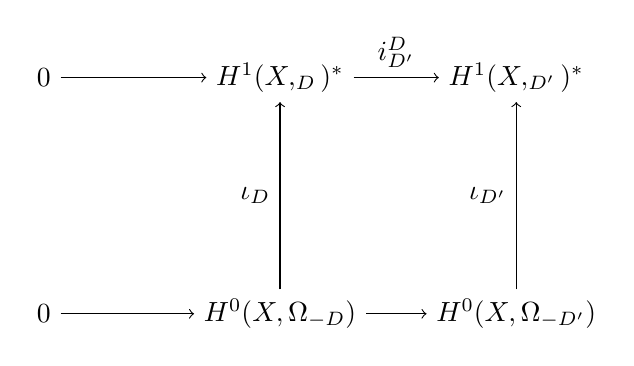
\begin{tikzpicture}[node distance=3cm, auto]
      \node (H1D) {$H^1(X, \hol_D)^\ast$};
      \node (H1D') [right of=H1D] {$H^1(X, \hol_{D'})^\ast$};
      \node (01) [left of=H1D] {0};
      \node (H0D) [below of=H1D] {$H^0(X, \Omega_{-D})$};
      \node (H0D') [right of=H0D] {$H^0(X, \Omega_{-D'})$};
      \node (02) [left of=H0D] {0};
      \draw[->] (01) to (H1D);
      \draw[->] (H1D) to node {$i_{D'}^D$} (H1D');
      \draw[->] (02) to (H0D);
      \draw[->] (H0D) to (H0D');
      \draw[->] (H0D) to node {$\iota_D$} (H1D);
      \draw[->] (H0D') to node {$\iota_{D'}$} (H1D');
    \end{tikzpicture}.
  \end{center}
\end{lemma}

\begin{proof}
  Wir wählen ein $\omega \in H^0(X, \Omega_{-D}) \subset H^0(X,
  \Omega_{-D'})$ und $\xi \in H^1(X, \hol_{D'})$. Dann gilt
  \[
  i_{D'}^D \circ \iota_D(\omega)(\xi) = \g{\omega}{\xi} =
  \iota_{D'}(\omega)(\xi).
  \]
\end{proof}

\begin{lemma}
  \label{lemma:urbilder}
  Sei die Notation wie in Lemma \ref{lemma:cd}. Seien weiterhin
  $\lambda \in H^1(X, \hol_D)^\ast$ und $\omega \in H^0(X,
  \Omega_{-D'})$ mit $i_{D'}^D(\lambda) = \iota_{D'}(\omega)$. Dann
  liegt $\omega$ bereits in $H^0(X, \Omega_{-D})$ und es ist $\lambda =
  \iota_D (\omega)$.
\end{lemma}

\begin{proof}
  Angenommen es gelte $\omega \notin H^0(X, \Omega_{-D}) \cong
  \Omega_{-D}(X)$. Dann existierte ein $a \in X$, so dass
  $\ord_a(\omega) < D(a)$ gelten müsste. Sei $(U_0, z)$ eine Koordinatenumgebung
  von $a$ mit $z(a) = 0$. Auf dieser Koordinatenumgebung drücken wir
  $\omega$ durch $\omega = f \d[z]$ mit einem $f \in \mer(U_0)$
  aus. Wir können ohne Einschränkung annehmen, dass wir $U_0$ klein
  genug gewählt haben, so dass
  \begin{enumerate}
  \item $D|_{U_0 \setminus \{a\}} = 0 = D'|_{U_0 \setminus
      \{a\}}$ gilt und
  \item $f$ keine Null- und Polstellen in $U_0 \setminus \{a\}$ besitzt.
  \end{enumerate}
  Nun setzen wir $U_1 := X \setminus \{a\}$, $\fu = (U_0, U_1)$ und
  $\eta = (f_0, f_1) \in C^0(\fu, \mer)$, wobei $f_0 := (zf)^{-1}$ und
  $f_1 := 0$ definiert wird. Aus $\ord_a(\omega) < D(a)$ folgte nun
  sogar, dass $\eta \in C^0(\fu, \hol_D)$ und damit, dass
  \[
  \delta \eta \in Z^1(\fu, \hol) = Z^1(\fu, \hol_D) = Z^1(\fu,
  \hol_{D'})
  \]
  gelten müsste. Bezeichnen wir mit $\xi'$ die
  Kohomologieklasse von $\delta \eta$ in $H^1(X, \hol_{D'})$ und mit
  $\xi$ die Kohomologieklasse von $\delta \eta$ in $H^1(X, \hol_D)$,
  so erhalten wir zunächst, weil \break$\eta \in C^0(\fu, \hol_D)$ ist, dass
  $\xi = 0$ gilt. Nach Voraussetzung gälte nun aber
  \[
  \g{\omega}{\xi'} = \iota_{D'}(\omega)(\xi') =
  i_{D'}^D(\lambda)(\xi') = \lambda(\xi) = 0.
  \]
  Andererseits ist $\omega \eta = \left ( \frac{\d[z]}{z}, 0 \right )$
  und es folgt
  \[
  \g{\omega}{\xi'} = \res(\omega \eta) = 1.
  \]
  Ein Widerspruch. Also muss $\omega \in H^0(X, \Omega_{-D})$
  gelten. Da dann
  \[
  i_{D'}^D(\lambda) = \iota_{D'}(\omega) = i_{D'}^D(\iota_D(\omega))
  \]
  gelten muss, folgt $\lambda =
  \iota_D(\omega)$ aus der Injektivität von $i_{D'}^D$.
\end{proof}

\begin{lemma}
  Seien $X$ eine kompakte Riemannsche Fläche und $D,B \in \Div(X)$.
  Sei \break $\psi \in H^0(X,\hol_B)$. Dann induziert der
  Garbenhomomorphismus
  \[
  \hol_{D-B} \xrightarrow{\psi} \hol_D, \quad f \mapsto \psi f
  \] 
  eine lineare Abbildung
  \[
  H^1(X, \hol_{D-B}) \ra H^1(X, \hol_D)
  \]
  und damit auch eine lineare Abbildung
  \[
  H^1(X, \hol_D)^\ast \ra H^1(X, \hol_{D-B})^\ast.
  \]
  Diese bezeichnen wir auch mit $\psi$. Mit dieser Notation folgt
  $(\psi \lambda)(\xi) = \lambda(\psi \xi)$ für beliebige $\lambda \in
  H^1(X, \hol_D)^\ast$ und $\xi \in H^1(X, \hol_{D-B})$. Weiterhin
  kommutiert das folgende Diagramm
  \begin{center}
    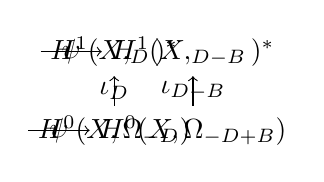
\begin{tikzpicture}
      \node (H1D) {$H^1(X, \hol_D)^\ast$};
      \node (H1B) [right of=H1D] {$H^1(X, \hol_{D-B})^\ast$};
      \node (H0D) [below of=H1D] {$H^0(X, \Omega_{-D})$};
      \node (H0B) [right of=H0D] {$H^0(X, \Omega_{-D +B})$};
      \draw[->] (H1D) to node {$\psi$} (H1B);
      \draw[->] (H0D) to node {$\psi$} (H0B);
      \draw[->] (H0D) to node {$\iota_D$} (H1D);
      \draw[->] (H0B) to node {$\iota_{D-B}$} (H1B);
    \end{tikzpicture}.
  \end{center}
\end{lemma}

\begin{proof}
  Dass Multiplikation mit $\psi$ ein Garbenhomomorphismus ist, ist klar
  und damit folgt die Existenz der linearen Abbildungen. Die
  Kommutativität des Diagramms erhalten wir aus der Tatsache, dass wir
  für beliebige $\omega \in H^0(X, \Omega_{-D})$ und $\xi \in H^1(X,
  \hol_{D-B})$ die folgende Rechnung durchführen können
  \begin{align*}
    \iota_{D-B}(\psi \omega)(\xi) = \g{\psi \omega}{\xi} = \res((\psi
    \omega) \xi) = \res(\omega (\psi \xi)) = \g{\omega}{\psi \xi} =
    \iota_D(\omega)(\psi \xi).
  \end{align*}
\end{proof}

\begin{lemma}
  \label{lemma:psi-inj}
  Falls $\psi \in H^0(X, \hol_B)$ mit $\psi \neq 0$ gilt, so ist
  \[
  \psi: H^1(X, \hol_D)^\ast \ra H^1(X, \hol_{D-B})^\ast
  \]
  injektiv.
\end{lemma}

\begin{proof}
  Sei $A := (\psi) \geq -B$. Dann faktorisiert $\psi: \hol_{D-B} \ra
  \hol_D$ über $\hol_{D+A}$, d.h. das Diagramm
  \begin{center}
    \begin{tikzpicture}[node distance = 1.5cm, auto]
      \node (DB) {$\hol_{D-B}$};
      \node (D) [right of=DB] {$\hol_D$};
      \node (A) [below of=DB] {$\hol_{D+A}$};
      \draw[->] (DB) to node {$\psi$} (D);
      \draw[->] (DB) to (A);
      \draw[->, dashed] (A) to (D);
    \end{tikzpicture}
  \end{center}
  kommutiert. Weiterhin ist die Abbildung $\hol_{D+A} \ra \hol_D$ ein
  Isomorphismus, wobei die Umkehrung einfach durch Multiplikation mit
  $\psi^{-1}$ gegeben ist. Nun ist die Inklusion von $\hol_{D-B} \ra
  \hol_{D+A}$ injektiv und deshalb nach \cite[Satz 16.8]{For}
  \[
  H^1(X, \hol_{D-B}) \ra H^1(X, \hol_{D+A})
  \]
  ein Epimorphismus. Also ist auch
  \[
  H^1(X,\hol_{D-B}) \xrightarrow{\psi} H^1(X, \hol_D)
  \]
  ein Epimorphismus und schlußendlich die duale Abbildung
  injektiv. Dies zeigt die Behauptung.
\end{proof}

\begin{thm}[Der Serresche Dualitätssatz]
  \label{thm:serre}
  Sei $D \in \Div(X)$ und $X$ eine kompakte Riemannsche Fläche. Dann
  ist $\iota_D: H^0(X, \Omega_{-D}) \ra H^1(X, \hol_D)^\ast$ ein Isomorphismus.
\end{thm}

\begin{proof}
  Aufgrund von Satz \ref{thm:iota-inj} benötigen wir nur noch die
  Surjektivität von $\iota_D$. Sei \break$\lambda \in H^1(X, \hol_D)^\ast$
  mit $\lambda \neq 0$ und $P \in \Div(X)$ mit $\deg P = 1$. Weiterhin
  setzen wir $D_n := D - n P$ für beliebige $n \in \N$. Als nächstes
  bezeichnen wir mit $\Lambda \subset H^1(X, \hol_{D_n})^\ast$ den
  Untervektorraum aller Linearformen der Form $\psi \lambda$ mit
  $\psi \in H^0(X, \hol_{nP})$. Nach Lemma \ref{lemma:psi-inj} gilt
  $\Lambda \cong H^0(X, \hol_{nP})$. Aus dem Satz von Riemann-Roch
  folgt damit
  \[
  \dim \Lambda \geq 1 - g + n.
  \]
  Lemma \ref{lemma:k0} und die Injektivität von $\iota_{D_n}$ implizieren
  \[
  \dim \im(\iota_{D_n}) = \dim H^0(X, \Omega_{-D_n}) \geq n + k_0 -
  \deg D.
  \]
  Wählen wir $n > \deg D$, so erhalten wir $\deg D_n < 0$ und damit
  $H^0(X, \hol_{D_n}) = 0$ nach \cite[Satz 16.5]{For}. Aus dem Satz von Riemann-Roch folgt
  \[
  \dim H^1(X, \hol_{D_n})^\ast = g - 1 - \deg D_n = n + ( g - 1 -
  \deg D).
  \]
  Unter eventueller Vergrößerung von $n$ erhalten wir
  \begin{align*}
    \dim \Lambda + \dim \im(\iota_{D_n}) & \geq 1 - g + n + n + k_0 -
    \deg D \\
    & = 2 n + 1 - g + \deg D \\
    & > n + (g - 1 - \deg D) \\
    & = \dim H^1(X, \hol_{D_n})^\ast.
  \end{align*}
  Da sowohl $\Lambda$ als auch $\im(\iota_{D_n})$ Untervektorräume von
  $H^1(X, \hol_{D_n})^\ast$ sind, muss
  \[
  \Lambda \cap \im(\iota_{D_n}) \neq 0
  \]
  sein. Also existiert ein $\psi \in H^0(X, \hol_{nP})$ mit
  $\psi \neq 0$ und ein $\omega \in H^0(X, \Omega_{-D_n})$ mit $\psi
  \lambda = \iota_{D_n}(\omega)$. Setzen wir $A := (\psi)$, so liegt
  $\frac{1}{\psi}$ in $H^0(X, \hol_A)$. Zu guter Letzt erhalten wir aus
  $D' := D_n - A$, dass
  \begin{align*}
    i_{D'}^D(\lambda) = \frac{1}{\psi} (\psi \lambda) =
    \frac{1}{\psi} \iota_{D_n}(\omega) = \iota_{D'} \left (
      \frac{1}{\psi} \omega \right )
  \end{align*}
  gilt und unter Ausnutzung von Lemma \ref{lemma:urbilder} folgt, dass
  $\omega_0 := \frac{1}{\psi} \omega \in H^0(X, \Omega_{-D})$ die
  Gleichung $\lambda = \iota_D(\omega_0)$ erfüllt.
\end{proof}

\begin{cor}
  \label{cor:dim-1-form}
  Sei $X$ eine kompakte Riemannsche Fläche und $D \in \Div(X)$. Dann
  gilt
  \[
  \dim H^1(X, \hol_D) = \dim H^0(X, \Omega_{-D}).
  \]
  Insbesondere folgt für $D = 0$
  \[
  g = \dim H^1(X, \hol) = \dim H^0(X, \Omega),
  \]
  wobei $g$ das Geschlecht von $X$ bezeichnet.
\end{cor}

\begin{thm}
  \label{thm:serre-umgekehrt}
  Sei $D \in \Div(X)$ und $X$ eine kompakte Riemannsche Fläche. Dann
  gilt
  \[
  H^0(X, \hol_{-D}) \cong H^1(X, \Omega_D)^\ast.
  \]
\end{thm}

\begin{proof}
  Sei $0 \neq \omega_0 \in \mer^{(1)}(X)$ und $K := (\omega_0)$. Wie
  aus Definition \ref{def:garbe-div} bekannt, gelten $\Omega_D \cong
  \hol_{D+K}$ und $\hol_D \cong \Omega_{-D-K}$. Mit Satz
  \ref{thm:serre} folgt
  \[
  H^0(X, \hol_{-D}) \cong H^0(X, \Omega_{-D-K}) \cong H^1(X,
  \hol_{D+K})^\ast = H^1(X, \Omega_D)^\ast.
  \]
\end{proof}

\begin{cor}
  \label{cor:hol-form}
  Sei $X$ eine kompakte Riemannsche Fläche. Dann gilt $\dim H^1(X,
  \Omega) = 1$.
\end{cor}

\begin{proof}
  Satz \ref{thm:serre-umgekehrt} angewandt auf den Fall $D = 0$
  liefert uns
  \[
  \dim H^1(X, \Omega) = \dim H^0(X, \hol) = \dim \C = 1.
  \]
\end{proof}

\begin{thm}
  \label{thm:deg-geschlecht}
  Sei $X$ eine kompakte Riemannsche Fläche mit Geschlecht $g$ und $\omega
  \in \mer^{(1)}(X)$, wobei $\omega(x) \neq 0$ für jedes $x \in
  X$. Dann gilt
  \[
  \deg(\omega) = 2g - 2.
  \]
\end{thm}

\begin{proof}
  Sei $K := (\omega)$. Aus dem Satz von Riemann-Roch erhalten wir
  \[
  \dim H^0(X, \hol_K) - \dim H^1(X, \hol_K) = 1 - g + \deg K.
  \]
  Wieder nach Definiton \ref{def:garbe-div} wissen wir $\Omega \cong
  \hol_K$. Also erhalten wir weiter unter Ausnutzung von Satz
  \ref{thm:serre} und Korollar \ref{cor:hol-form} die folgende Gleichung
  \begin{align*}
    1 - g+ \deg K & = \dim H^0(X, \Omega) - \dim H^1(X, \Omega) \\
    & = \dim H^1(X, \hol) - 1 \\
    & = g - 1.
  \end{align*}
  Aufgelöst nach $\deg K$ folgt die Behauptung.
\end{proof}

\begin{defin}
  \label{defin:gitter}
  Sei $V$ ein $n-$dimensionaler, reeller Vektorraum. Eine additive
  Untergruppe $\Gamma \subset V$ heißt \init{Gitter}, falls $n$ linear
  unabhängige $\gamma_1, \dots, \gamma_n \in V$ existieren, so dass
  \[
  \Gamma = \Z \gamma_1 + \dots + \Z \gamma_2
  \]
  gilt.
\end{defin}

\begin{cor}
  \label{cor:torus-geschlecht}
  Sei $\Gamma \subset \C$ ein Gitter. Dann hat der Torus
  $\quot{\C}{\Gamma}$ Geschlecht 1.
\end{cor}

\begin{proof}
  Wir betrachten die meromorphe 1-Form $\d[z]$ auf $\C$. Da $\C$ die
  Universelle Überlagerung von $\quot{\C}{\Gamma}$ darstellt und wir
  deshalb die Projektion als Kartenabbildung von $\quot{\C}{\Gamma}$
  verwenden können, finden wir eine 1-Form $\omega \in
  \quot{\C}{\Gamma}$, die auf jeder dieser Karten mit $\d[z]$
  übereinstimmt. Dann folgt aber sofort $\omega(x) \neq 0$ für jedes $x
  \in \quot{\C}{\Gamma}$ und damit $\deg(\omega) = 0$. Aus Satz
  \ref{thm:deg-geschlecht} folgt dann $g = 1$.
\end{proof}


Korollar \ref{cor:dim-1-form} und \ref{cor:torus-geschlecht} finden
direkt Anwendung im Beweis des Uniformisierungssatzes
\ref{thm:uniformisierung}. Die folgenden Kapitel wenden sich nun aber
hauptsächlich \emph{nicht} kompakten Riemannschen Flächen zu, so dass
die Resultate dieses Kapitels zwar immer im Hinterkopf behalten werden
sollten, aber in den nächsten Kapiteln keine Rolle spielen.

%%% Local Variables: 
%%% mode: latex
%%% TeX-master: "../Bachelor"
%%% End: 

